\documentclass[twocolumn]{iopjournal}

\usepackage{amsmath,amssymb,amsfonts,amsthm,graphicx}

\fancyhfoffset[L]{0mm}
\setlength{\marginparwidth}{0pt}
\setlength{\marginparsep}{0pt}

\renewcommand{\articletype}[1]{%
  {\vspace*{-8mm}\noindent \Large \sf Preprint}\par
  \vspace*{6mm}\noindent{\scriptsize \sf{\bfseries \MakeUppercase{#1}}}}

\fancyhead[L]{}
\fancyhead[R]{}

\hypersetup{pdftitle={The Mountain Scale in the SST: the Net-Field Rule From the Action}, pdfauthor={Stephen Nelson}, pdfsubject={Gravity Field Dynamics (GFD)}, pdfkeywords={SST, net-field rule, mountain scale, Jacobi radius, projector, preferred foliation, action, MOND, proof}}

\begin{document}

\articletype{Supplementary Material}

\title{The Mountain Scale in the SST: the Net-Field Rule From the Action}

\author{Stephen Nelson}

\affil{Field Dynamics Research}

\ead{stephen@fielddynamics.org}

\begin{abstract}
\emph{The picture.} A mountain stream looks flat close up; zoomed out,
it runs down a mountain. Inside a bound system the host's field is a
flat slope, and each body is a dimple with no drain; seen from outside,
the whole mountain shows, and the constitutive law acts on it. The two
views meet at the system's Jacobi radius.

This note writes the picture into the action. The SST has a preferred
foliation~\cite{NelsonTL}, so on each leaf there is a projector $P$
onto spatial modes longer than the mountain scale $\ell$: the spectral
projector of the leaf's Laplacian, self-adjoint, idempotent and
covariant under the foliation's symmetry. The curvature term is read
at every point, as in general relativity; the law's term is read on
the mountain's lapse, $P\Phi$. The field equation then splits exactly:
the dimple $\Phi - P\Phi$ obeys Poisson's equation with
$(1 - P)\rho$, linear, pure TetA with the bare $G$, whatever the law;
the mountain $P\Phi$ obeys the law at the mountain's scale. This is
the net-field rule's two-scale split, now derived from an action. The
tail is gone, $\gamma = 1$ and the galaxy results are unchanged, and
the khronon sector of the dimple is empty, as the khronon proof
required. The data fix the mountain scale: it is each bound system's
own Jacobi radius ($1.4$~pc for the Sun, $\sim160$ and $\sim270$~pc for
Pal~14 and Pal~4), not one universal length. A 3D solution confirms
the split, the missing tail and the unchanged galaxy.
\end{abstract}

\keywords{SST, net-field rule, mountain scale, Jacobi radius, projector, preferred foliation, action, MOND, proof}

% ----------------------------------------------------------------------

\section*{Setting}

The SST~\cite{NelsonTL}, varied as the framework varies it, is
$(1/16\pi G)\sqrt{-g}[R - 2f(a)] - \tfrac14e^{-2\Phi/c^2}F^2 +
\mathcal L_{\rm m}$ with $f = a_0^2[F(y) - y]$,
$F(y) = y - 2\sqrt y + 2\ln(1+\sqrt y)$, $y = c^4a_\mu a^\mu/a_0^2$, and
$a$ the acceleration of the tetrad's time leg, normal to a preferred
foliation. In a static metric $a_i = \partial_i\ln N$ and
$\Phi = c^2\ln N$ is the lapse potential. Read point by point, this
action applies the law to every body's own field and leaves the tail
$(1-\mu)g = a_0\mu \to a_0$~\cite{NelsonTL,NelsonKh}, which perihelia
exclude. The net-field rule~\cite{NelsonNFR} removes it by reading the
law on the galaxy's coarse-grained field; the khronon proof showed the
preferred frame obeys the same picture~\cite{NelsonKh}. Both left the
same step open: writing ``at the mountain's scale'' into the action.

Every statement below is checked by the accompanying script (17
checks) and a 3D solution~\cite{NelsonScript}; the split is
machine-checked in Lean~4 (3 theorems, importing the khronon and
net-field formalisations).

% ----------------------------------------------------------------------

\section*{Definition (the mountain scale in the action)}

On each leaf $\Sigma_t$ of the preferred foliation, with induced metric
$h$ and Laplace--Beltrami operator $\Delta_h$, let
\begin{equation}
P_\ell = \Theta\big((\pi/\ell)^2 + \Delta_h\big),
\label{eq:P}
\end{equation}
the spectral projector onto the modes of $-\Delta_h$ with eigenvalue at
most $(\pi/\ell)^2$: wavelengths longer than $2\ell$. Define the
mountain's lapse and its time leg's acceleration,
\begin{equation}
\bar N = e^{P_\ell\Phi/c^2},\quad \bar a_i = \partial_i\ln\bar N,\quad
\bar y = \frac{c^4\bar a\cdot\bar a}{a_0^2},
\label{eq:bar}
\end{equation}
and take the action
\begin{equation}
\begin{aligned}
S = \!\int\! d^4x\sqrt{-g}\Big[&\frac{R - 2a_0^2[F(\bar y) - \bar y]}{16\pi G}\\
&- \tfrac14e^{-2\Phi/c^2}F^2 + \mathcal L_{\rm m}\Big].
\end{aligned}
\label{eq:S}
\end{equation}
The curvature term, which carries all of Newton and Einstein, is read
at every point. Only the law's term, the TetB share, is read at the
mountain's scale.

$P_\ell$ is self-adjoint in the leaf's volume measure, idempotent, and
commutes with $\Delta_h$; it is defined by the leaf geometry alone, so
it is covariant under the foliation-preserving diffeomorphisms, the
symmetry of a theory with a preferred foliation (script B1, on a
randomly curved leaf). It acts within each leaf, instantaneously in the
preferred time, as the elliptic constraints of khronometric theories
do.

% ----------------------------------------------------------------------

\section*{Theorem 1 (the field equation)}

\emph{In the static weak field, with $\bar\Phi = P\Phi$ and
$4\pi G\rho$ the source, the Lagrangian is
$-|\nabla\Phi|^2/8\pi G - \rho\Phi - (a_0^2/8\pi G)[F(\bar y) - \bar y]$,
and its field equation is
\begin{equation}
\nabla^2\Phi + P\,\nabla\cdot\big[(\bar\mu - 1)\nabla\bar\Phi\big]
= 4\pi G\rho,
\label{eq:EL}
\end{equation}
with $\bar\mu = \mu(|\nabla\bar\Phi|/a_0)$. The curvature term's $\Psi$-equation is unchanged, so $\Psi = \Phi$
($\gamma = 1$).}

\begin{proof}
Vary $\Phi$; the chain rule through $\bar\Phi = P\Phi$ brings back
$P^\dagger = P$, and $\partial_y[F - y] = \mu - 1$. Checked: the
finite-difference gradient of the discrete action equals~(\ref{eq:EL})
in 1D (script A2) and in 3D (E1).
\end{proof}

% ----------------------------------------------------------------------

\section*{Theorem 2 (the exact split)}

\emph{Because $P$ is idempotent and commutes with $\nabla$,
(\ref{eq:EL}) splits into
\begin{align}
\nabla^2(\Phi - P\Phi) &= 4\pi G\,(1 - P)\rho, \label{eq:dimple}\\
P\,\nabla\cdot\big[\bar\mu\,\nabla\bar\Phi\big] &= 4\pi G\,P\rho.
\label{eq:mountain}
\end{align}
The dimple~(\ref{eq:dimple}) is linear, with the bare $G$, and is the
same for every law: pure TetA. The mountain~(\ref{eq:mountain}) obeys
the law at the mountain's scale. Together,
$g = g_{\rm law}[P\rho] + g_N[(1 - P)\rho]$: the net-field rule's
two-scale split~\cite{NelsonNFR}, now a consequence of the action.}

\begin{proof}
Apply $1 - P$ and $P$ to~(\ref{eq:EL}), using $P^2 = P$ and
$P\nabla^2 = \nabla^2P$ (Lean \texttt{mountain\_split}); if $\nabla^2$ is
injective on the field space, the dimple depends on $\rho$ alone (Lean
\texttt{dimple\_blind\_to\_law}). Checked numerically: in 1D the dimple
equals the Newtonian potential of $(1-P)\rho$ to $4\times10^{-13}$, and
solving with a different law changes the mountain by 8\% and the
dimple not at all (script A3--A5); in 3D to $2\times10^{-15}$ (E1).
\end{proof}

% ----------------------------------------------------------------------

\section*{Theorem 3 (what follows)}

\emph{(a) No tail: the dimple's own law is linear, so its TetB share
is zero; read pointwise it would be $a_0\mu(x) > 0$ at every finite
field. (b) The galaxy is unchanged: the mountain is the galaxy seen at
resolution $\ell$. In 3D the galaxy's field differs from the pointwise
reading by $4\times10^{-2}$, $3\times10^{-3}$ and $2\times10^{-4}$ for
$\ell$ at 2, 1 and $\tfrac12$ of the galaxy's width; in the Milky Way
$\ell/R \sim 1.4\,{\rm pc}/8\,{\rm kpc} \sim 2\times10^{-4}$.
(c) $\gamma = 1$ and lensing mass equals dynamical mass, as
before~\cite{NelsonTL}. (d) The khronon: $f$ depends on $\bar y$ only,
so preferred-time perturbations on scales below $\ell$ drop out of
$f$; the dimple carries no khronon inertia, density or momentum, and
$\alpha_1 = \alpha_2 = 0$ inside a star system. This is the khronon
proof's Theorem~6~\cite{NelsonKh}, now derived rather than assumed.}

\begin{proof}
(a) Lean \texttt{no\_tail\_in\_dimple}. (b)--(d) from
Theorems~1--2 and~\cite{NelsonKh}; (a) and (b) are confirmed in 3D
(Fig.~\ref{fig:demo}; script E2--E4).
\end{proof}

\begin{figure}[t]
\centering
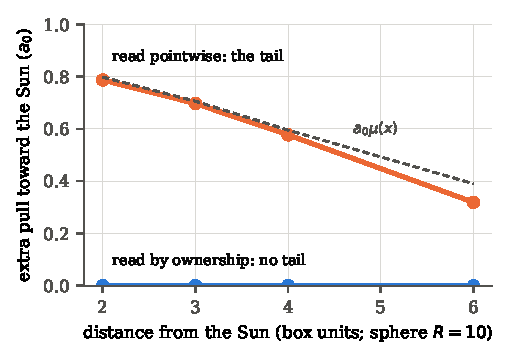
\includegraphics[width=\columnwidth]{fig_demo.pdf}
\caption{A 3D solution: a galaxy and a compact ``Sun'' in a periodic
box ($4\pi G = a_0 = 1$, mountain scale $\ell = 12$). The extra pull
toward the Sun beyond its own Newtonian pull, at distance $r$. Read
pointwise (orange) it is the tail, matching $a_0\mu(x)$ (line). Read at
the mountain's scale (blue) it is small and fades toward the Sun: only
the smoothed sheet and the tide. Script:
\texttt{demo\_mountain\_scale.py}.}
\label{fig:demo}
\end{figure}

% ----------------------------------------------------------------------

\section*{Proposition 4 (the mountain scale is the Jacobi radius)}

\emph{The data fix $\ell$, and it is each bound system's own Jacobi
radius, $r_J^3 = GM/2\Omega^2$, where the system's dimple meets the
host's tide:
\begin{enumerate}
\item the Sun: $r_J = 1.44$~pc, inside the net-field rule's window from
the Cassini bound ($1.2\times10^4$~AU $= 0.058$~pc) to binding;
\item Pal~14 ($1.2\times10^4\,M_\odot$, 71~kpc out): $r_J \approx
160$~pc, containing its 26~pc body; Pal~4: $r_J \approx 270$~pc,
containing its 18~pc body. Both are drainless dimples, Newton with
the bare $G$, as their dispersions require~\cite{NelsonNFR};
\item a single universal $\ell$ fails: at the Sun's $1.4$~pc, Pal~14's
body would lie in the mountain, its own field would be read through
the law, and in its external-field regime that is $G \to G/\mu$, the
factor the dispersions exclude at $8.9\sigma$~\cite{NelsonNFR}.
\end{enumerate}
So $P_\ell$ carries a position-dependent scale, $\ell(x) = r_J$ of the
bound system containing $x$. Theorems~1--3 are exact within each
system; where $\ell$ changes, at a Jacobi surface, the dimple's pull
equals the host's tide ($7\times10^{-14}$~m/s$^2$ for the Sun), which
bounds the departure there, and inside the system the net-field rule's
kernel bound $c(\nu-1)(r/\ell)^3$ applies ($4\times10^{-17}$ at
1~AU).}

\begin{proof}
Numbers checked (script D1--D4), with $v = 220$~km/s at the Sun and
$184$~km/s in the outer halo.
\end{proof}

In plain terms: the mountain scale is where your own dimple stops
standing out against the slope, and every bound system has its own.

% ----------------------------------------------------------------------

\section*{Scope}

Proved here: the mountain-scale action, its field equation, the exact
split into a linear dimple and a mountain that obeys the law, the
dimple's blindness to the law, the missing tail, $\gamma = 1$, the
derived khronon result, and the data's choice of scale.

Not proved here:
\begin{enumerate}
\item \emph{Why the edge follows the tide.} The Jacobi radius is fixed
by the picture and confirmed by the data; it is not derived from a
deeper principle.
\item \emph{The edges.} With $\ell(x)$ varying between systems, $P$ is
exact within each and bounded, not exact, at the Jacobi surfaces;
varying the action through the position of those surfaces is not
carried out.
\item \emph{Time-dependent binding.} Which bodies form a bound system,
and where its Jacobi surface lies, in mergers and tidal stripping.
\item \emph{Curved leaves.} $P$ commutes with $\Delta_h$ exactly, with
$\nabla$ only to $O(\Phi/c^2)$.
\end{enumerate}

% ----------------------------------------------------------------------

\begin{thebibliography}{99}

\bibitem{NelsonTL}
S.~Nelson,
\textit{The SST Covariant Completion: $y$ From the Acceleration of the
Time Leg} (2026), \texttt{proofs/sst-covariant-time-leg/}.

\bibitem{NelsonKh}
S.~Nelson,
\textit{The SST Khronon: Preferred-Frame Effects of the Time Leg}
(2026), \texttt{proofs/sst-khronon-preferred-frame/}.

\bibitem{NelsonNFR}
S.~Nelson,
\textit{The Net-Field Rule: Where the Constitutive Law Acts} (2026),
\texttt{proofs/net-field-rule/}.

\bibitem{NelsonScript}
S.~Nelson,
\texttt{verify\_sst\_mountain\_scale.py},
\texttt{demo\_mountain\_scale.py} and
\texttt{lean/MountainScale.lean} (2026),
\texttt{proofs/sst-mountain-scale/}.

\end{thebibliography}

\end{document}
